\begin{picture}(0,0)%
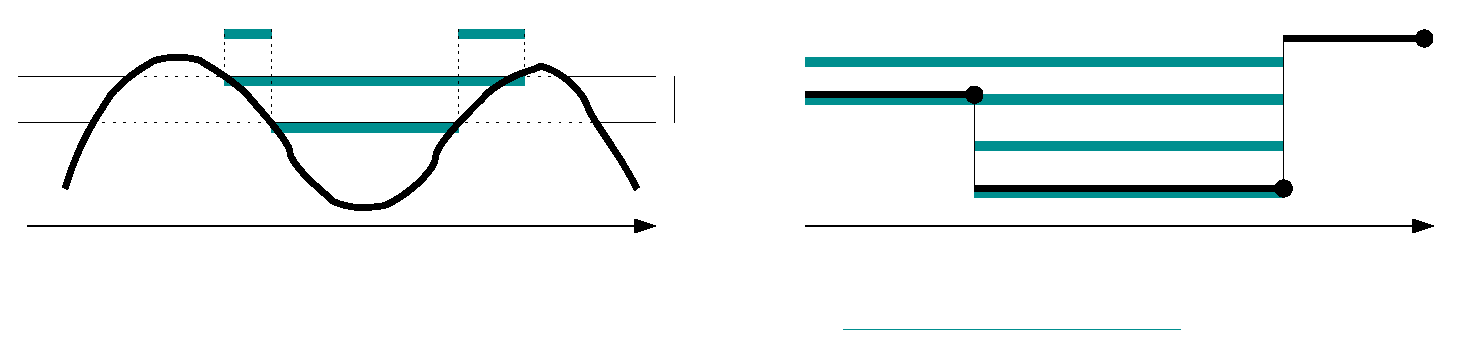
\includegraphics{doc/figures/mser-er-raw.ps}%
\end{picture}%
\setlength{\unitlength}{3947sp}%
%
\begingroup\makeatletter\ifx\SetFigFont\undefined%
\gdef\SetFigFont#1#2#3#4#5{%
  \reset@font\fontsize{#1}{#2pt}%
  \fontfamily{#3}\fontseries{#4}\fontshape{#5}%
  \selectfont}%
\fi\endgroup%
\begin{picture}(11511,2485)(2089,-3287)
\put(7426,-1561){\makebox(0,0)[lb]{\smash{{\SetFigFont{12}{14.4}{\familydefault}{\mddefault}{\updefault}{\color[rgb]{0,0,0}$\Delta$}%
}}}}
\put(2251,-2761){\makebox(0,0)[lb]{\smash{{\SetFigFont{12}{14.4}{\familydefault}{\mddefault}{\updefault}{\color[rgb]{0,0,0}Extremal regions are connected components of level sets.}%
}}}}
\put(4876,-1486){\makebox(0,0)[b]{\smash{{\SetFigFont{12}{14.4}{\familydefault}{\mddefault}{\updefault}{\color[rgb]{0,0,0}$R_{l+\Delta}$}%
}}}}
\put(4876,-1861){\makebox(0,0)[b]{\smash{{\SetFigFont{12}{14.4}{\familydefault}{\mddefault}{\updefault}{\color[rgb]{0,0,0}$R_l$}%
}}}}
\put(8401,-2761){\makebox(0,0)[lb]{\smash{{\SetFigFont{12}{14.4}{\familydefault}{\mddefault}{\updefault}{\color[rgb]{0,0,0}Discontinuities cause multiple extremal regions to coincide.}%
}}}}
\put(2251,-3016){\makebox(0,0)[lb]{\smash{{\SetFigFont{12}{14.4}{\familydefault}{\mddefault}{\updefault}{\color[rgb]{0,0,0}Extremal regions variation is used to compute stability.}%
}}}}
\put(4951,-961){\makebox(0,0)[b]{\smash{{\SetFigFont{12}{14.4}{\familydefault}{\mddefault}{\updefault}{\color[rgb]{0,0,0}$\Delta A$}%
}}}}
\put(7126,-2236){\makebox(0,0)[lb]{\smash{{\SetFigFont{12}{14.4}{\familydefault}{\mddefault}{\updefault}{\color[rgb]{0,0,0}$I(x)$}%
}}}}
\put(12526,-1186){\makebox(0,0)[lb]{\smash{{\SetFigFont{12}{14.4}{\familydefault}{\mddefault}{\updefault}{\color[rgb]{0,0,0}$I(x)$}%
}}}}
\put(13501,-2536){\makebox(0,0)[lb]{\smash{{\SetFigFont{12}{14.4}{\familydefault}{\mddefault}{\updefault}{\color[rgb]{0,0,0}$x$}%
}}}}
\put(7276,-2536){\makebox(0,0)[lb]{\smash{{\SetFigFont{12}{14.4}{\familydefault}{\mddefault}{\updefault}{\color[rgb]{0,0,0}$x$}%
}}}}
\end{picture}%
